\newpage
\section{Question 1}
	
	\subsection{Perpendicular Distance Function}	%a
		\lstinputlisting{./code/Q1/perpdist.m}
		\pagebreak
	\subsection{Least Square Minimization Algorithm}	%b
		\lstinputlisting{./code/Q1/leastsqmin.m}
		\pagebreak
	\subsection{Line Segmentation Algorithm}	%c
		\lstinputlisting{./code/Q1/lineseg.m}
		\linebreak
		\newline
		\subsubsection{Test Fitting}
			The following images are saved plots of sample data plots of increasing complexity where the original data is plotted with a red 'x' and the blue line through it is the approximated line segments. The relevant test scripts can be found in Appendix A [1].
			It's interesting to note that the sideways v test faces some inaccuracy in the approximation due the restriction on not allowing the index end points to be considered "corners". This is one of the shortcomings of using such a simple method of resolving the "broken data set" situation. A method that minimises that error as well would be much more difficult to program and much more intricate to specific case dealing.
			\begin{figure}[position = here]
				\begin{centering}
					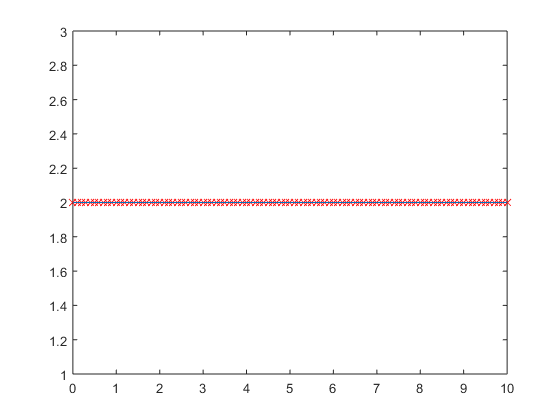
\includegraphics[scale=0.5]{q1_test00}\\
					\caption[\textit{RPYAxes}]{Horizontal Line}
				\end{centering}
			\end{figure}
			\newline
			
			\begin{figure}[position = here]
				\begin{centering}
					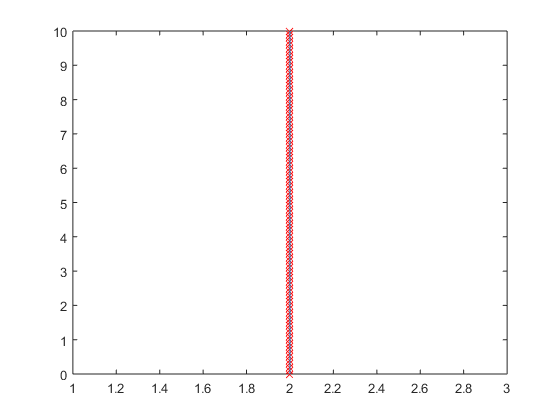
\includegraphics[scale=0.5]{q1_test01}\\
					\caption[\textit{RPYAxes}]{Vertical Line}
				\end{centering}
			\end{figure}
			\newline
			
			\begin{figure}[position = here]
				\begin{centering}
					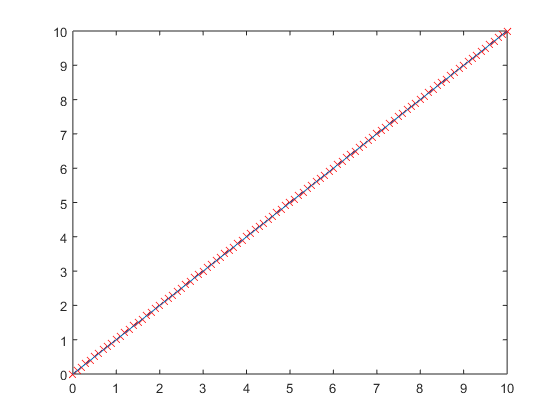
\includegraphics[scale=0.5]{q1_test02}\\
					\caption[\textit{RPYAxes}]{Slope (Through Origin)}
				\end{centering}
			\end{figure}
			\newline
			
			\begin{figure}[position = here]
				\begin{centering}
					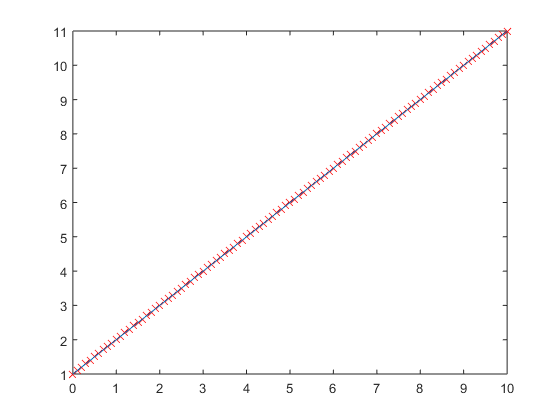
\includegraphics[scale=0.5]{q1_test03}\\
					\caption[\textit{RPYAxes}]{Offset Slope}
				\end{centering}
			\end{figure}
			\newline
			
			\begin{figure}[position = here]
				\begin{centering}
					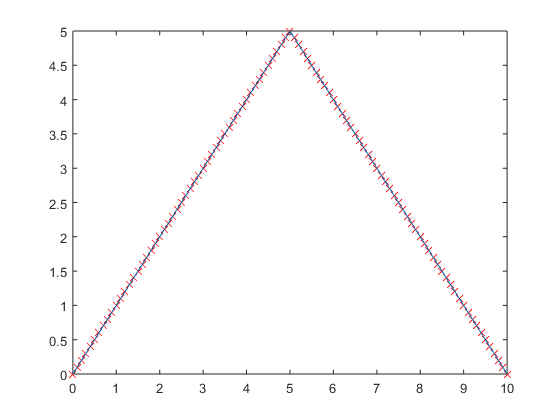
\includegraphics[scale=0.5]{q1_test04}\\
					\caption[\textit{RPYAxes}]{Inverted V}
				\end{centering}
			\end{figure}
			\newline			
			
			\begin{figure}[position = here]
				\begin{centering}
					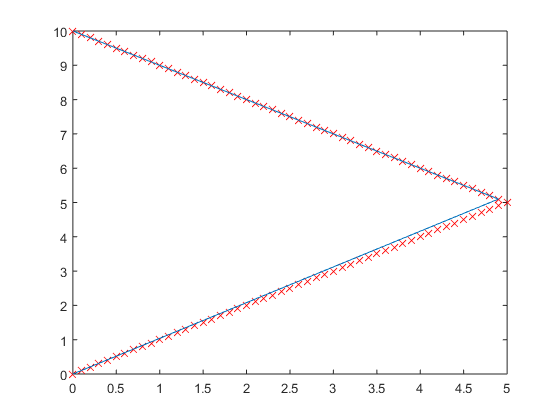
\includegraphics[scale=0.5]{q1_test05}\\
					\caption[\textit{RPYAxes}]{Sideways V}
				\end{centering}
			\end{figure}
			\newline			
			
			\begin{figure}[position = here]
				\begin{centering}
					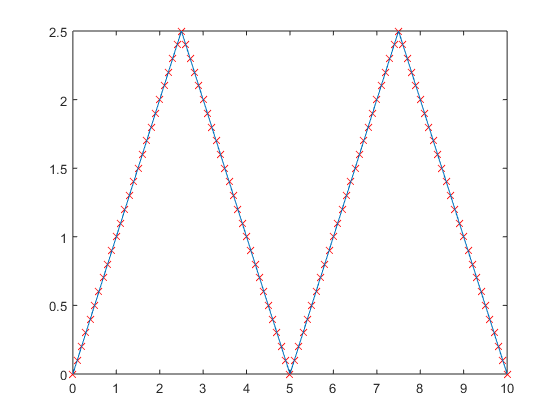
\includegraphics[scale=0.5]{q1_test06}\\
					\caption[\textit{RPYAxes}]{Perpendicular ZigZag)}
				\end{centering}
			\end{figure}
			\newline			
			
			\begin{figure}[position = here]
				\begin{centering}
					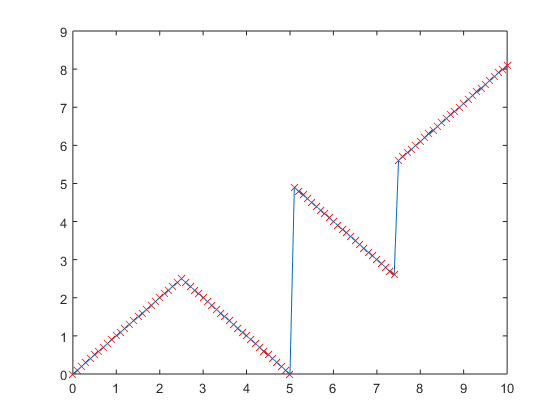
\includegraphics[scale=0.5]{q1_test07}\\
					\caption[\textit{RPYAxes}]{Broken Zig Zag}
				\end{centering}
			\end{figure}
			\newline			
			
			\begin{figure}[position = here]
				\begin{centering}
					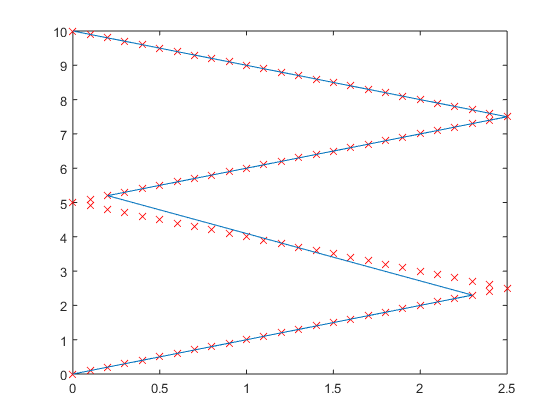
\includegraphics[scale=0.5]{q1_test08}\\
					\caption[\textit{RPYAxes}]{Perpendicular Zig Zag (Sideways)}
				\end{centering}
			\end{figure}
			\newline			
			
			\begin{figure}[position = here]
				\begin{centering}
					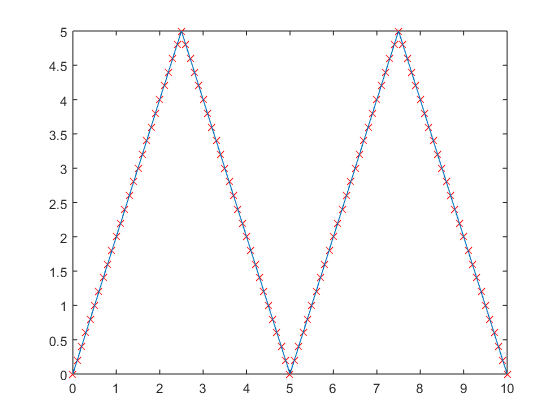
\includegraphics[scale=0.5]{q1_test09}\\
					\caption[\textit{RPYAxes}]{Non-Perpendicular ZigZag}
				\end{centering}
			\end{figure}
			\newline			
			
			\pagebreak
		\subsubsection{Test 06 Step by Step}
		The following images take a step by step plotted walk through on each estimation made on a simple case such as the Zig Zag pattern shown in test 06. The important thing to note is the recursive method utilised in this code which splits this into a logical problem solving technique (similar to mergesort or quicksort algorithms) by selecting pivot-points 
			\begin{figure}[position = here]
				\begin{centering}
					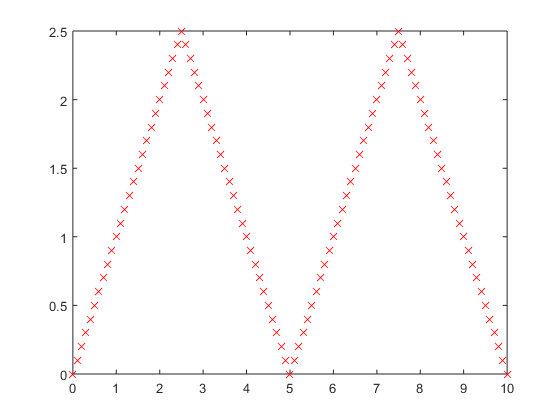
\includegraphics[scale=0.5]{q106_0}\\
					\caption[\textit{RPYAxes}]{Test 06 Stepped Through}
				\end{centering}
			\end{figure}
			\newline			
			
			\begin{figure}[position = here]
				\begin{centering}
					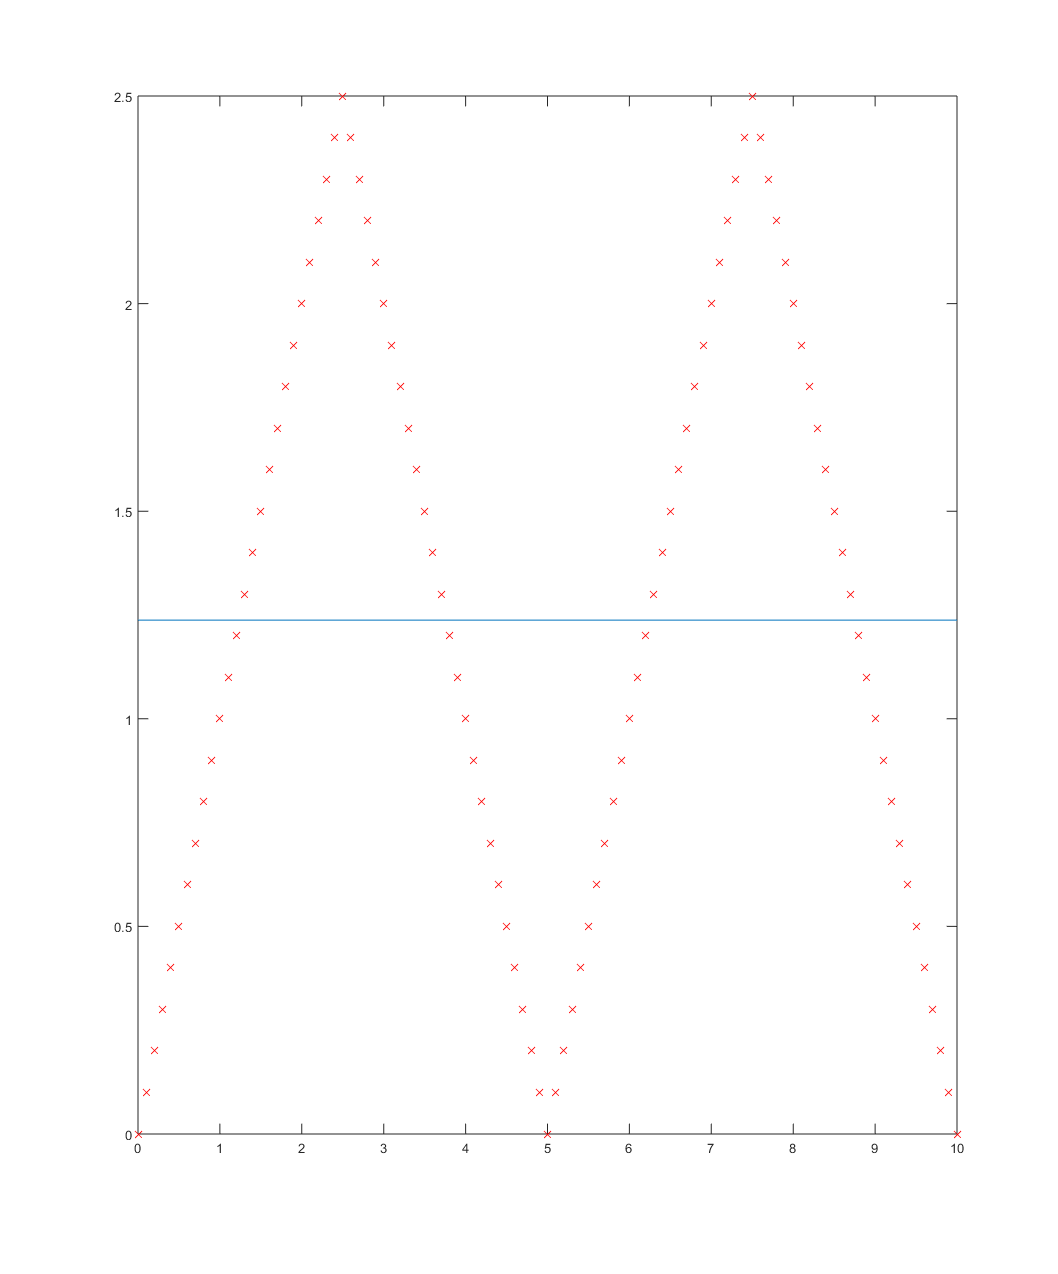
\includegraphics[scale=0.25]{q106_1}\\
					\caption[\textit{RPYAxes}]{Test 06 Stepped Through}
				\end{centering}
			\end{figure}
			\newline						

			\begin{figure}[position = here]
				\begin{centering}
					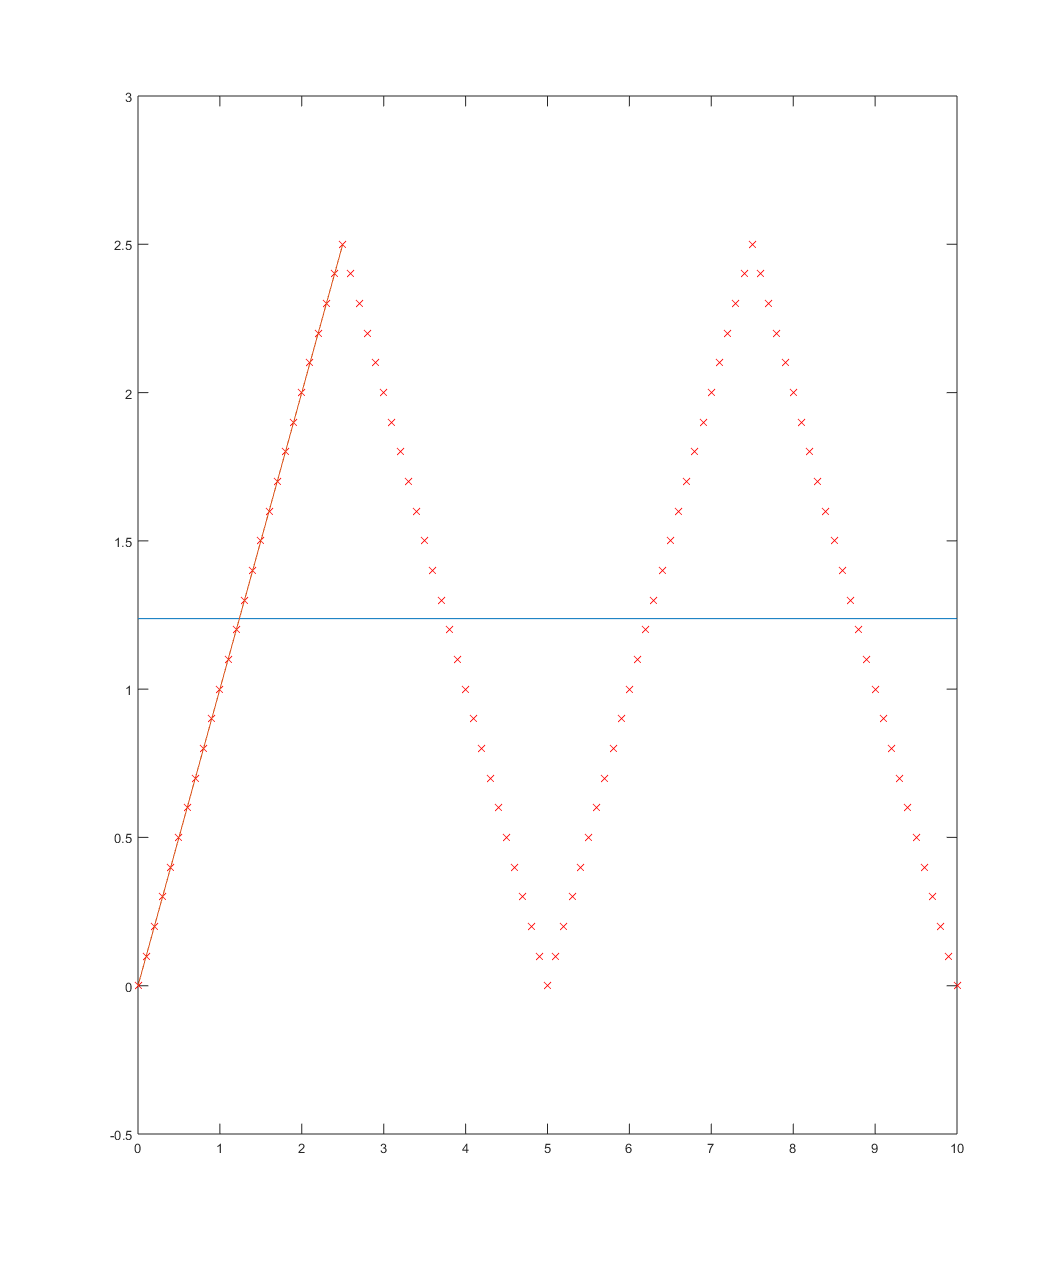
\includegraphics[scale=0.25]{q106_2}\\
					\caption[\textit{RPYAxes}]{Test 06 Stepped Through}
				\end{centering}
			\end{figure}
			\newline			
		
			\begin{figure}[position = here]
				\begin{centering}
					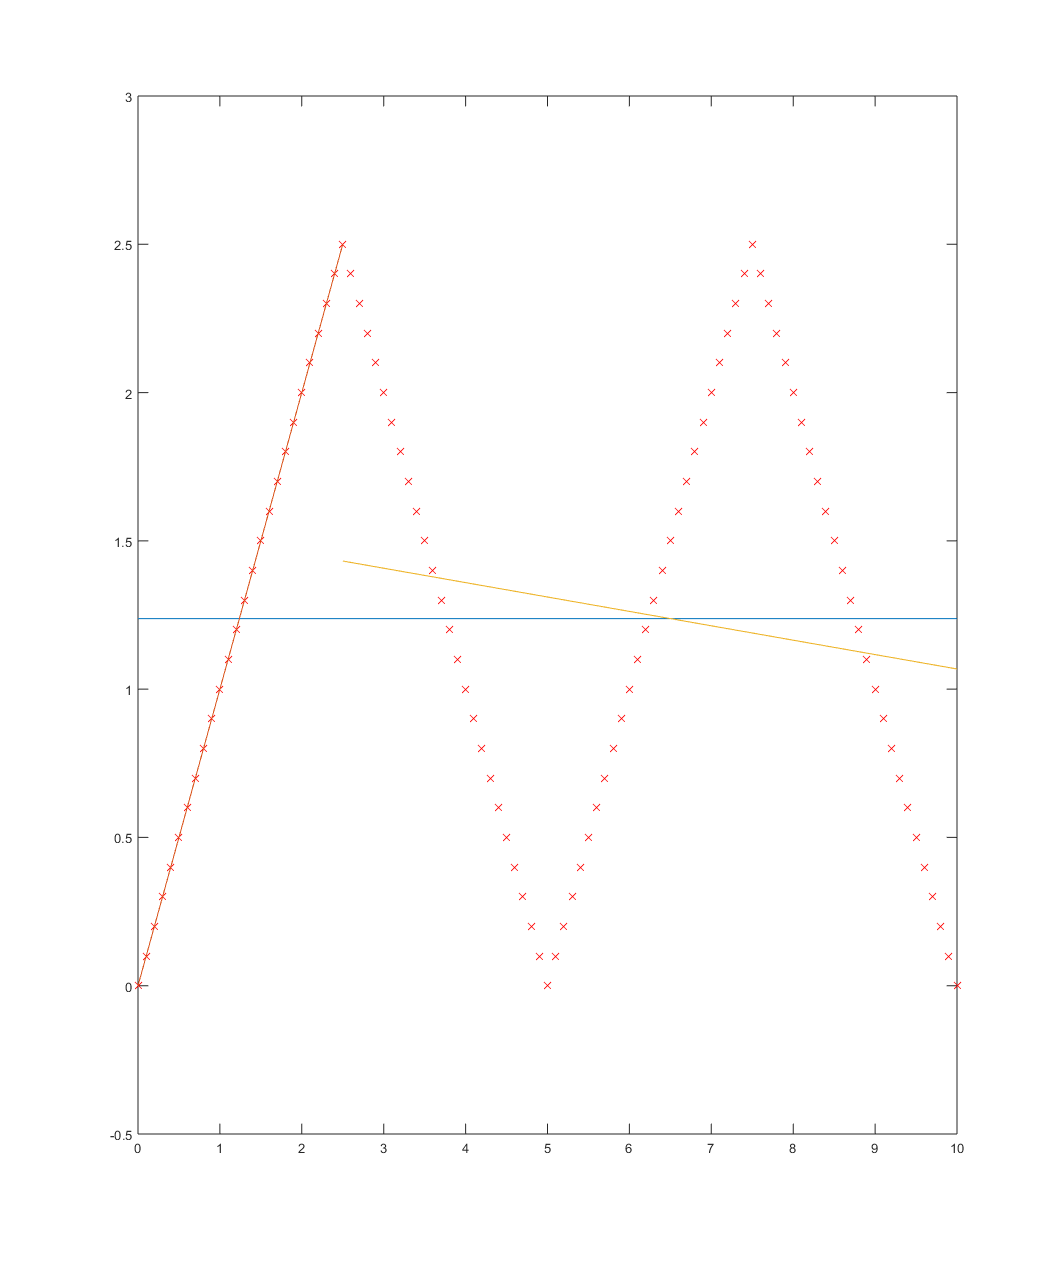
\includegraphics[scale=0.25]{q106_3}\\
					\caption[\textit{RPYAxes}]{Test 06 Stepped Through}
				\end{centering}
			\end{figure}
			\newline			
			
			\begin{figure}[position = here]
				\begin{centering}
					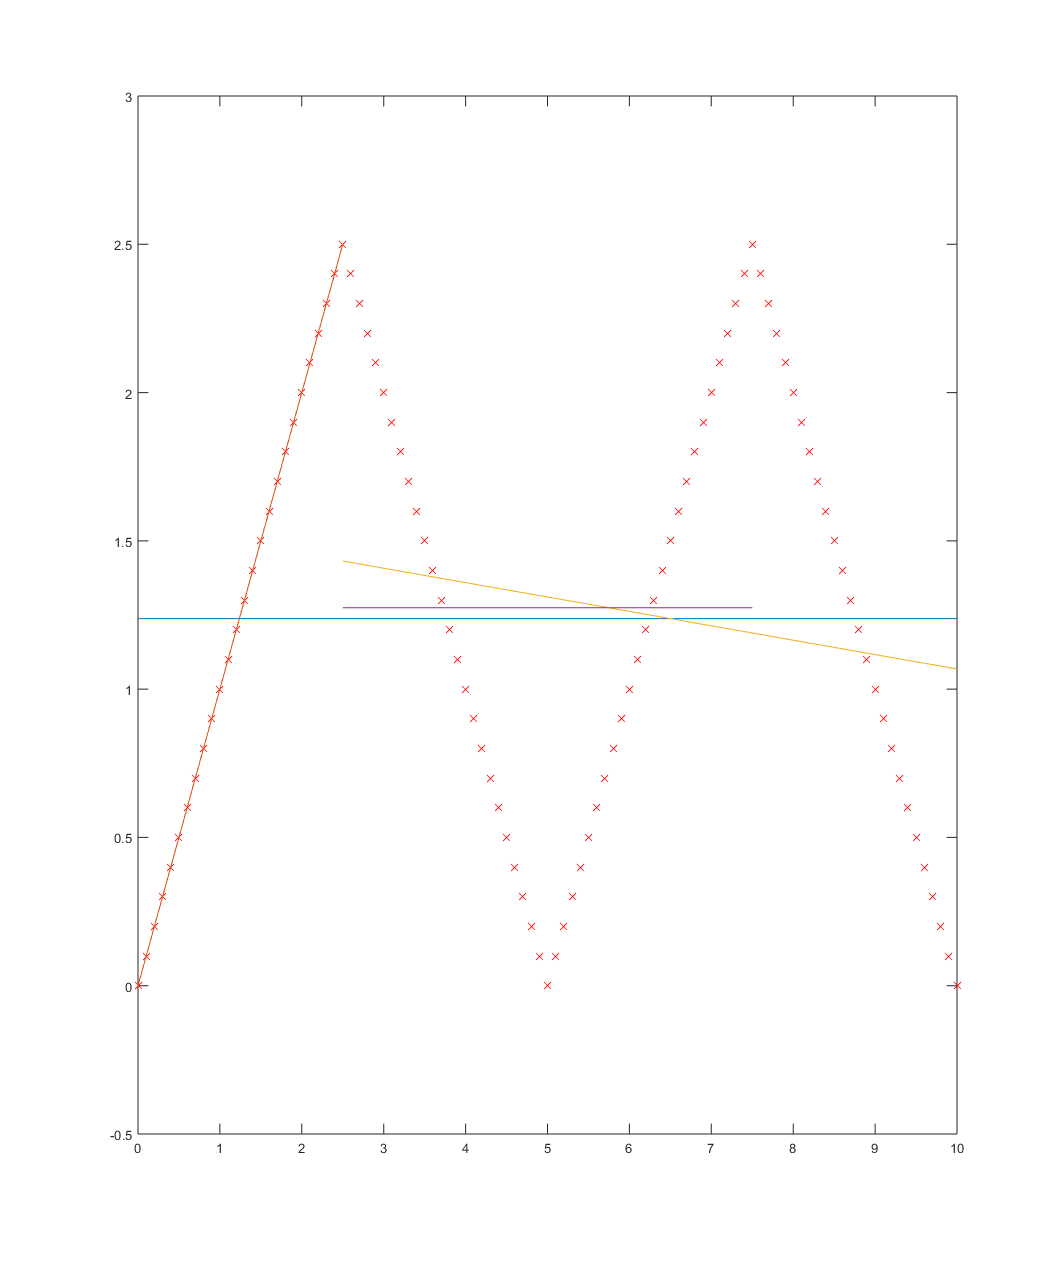
\includegraphics[scale=0.25]{q106_4}\\
					\caption[\textit{RPYAxes}]{Test 06 Stepped Through}
				\end{centering}
			\end{figure}
			\newline			
			
			\begin{figure}[position = here]
				\begin{centering}
					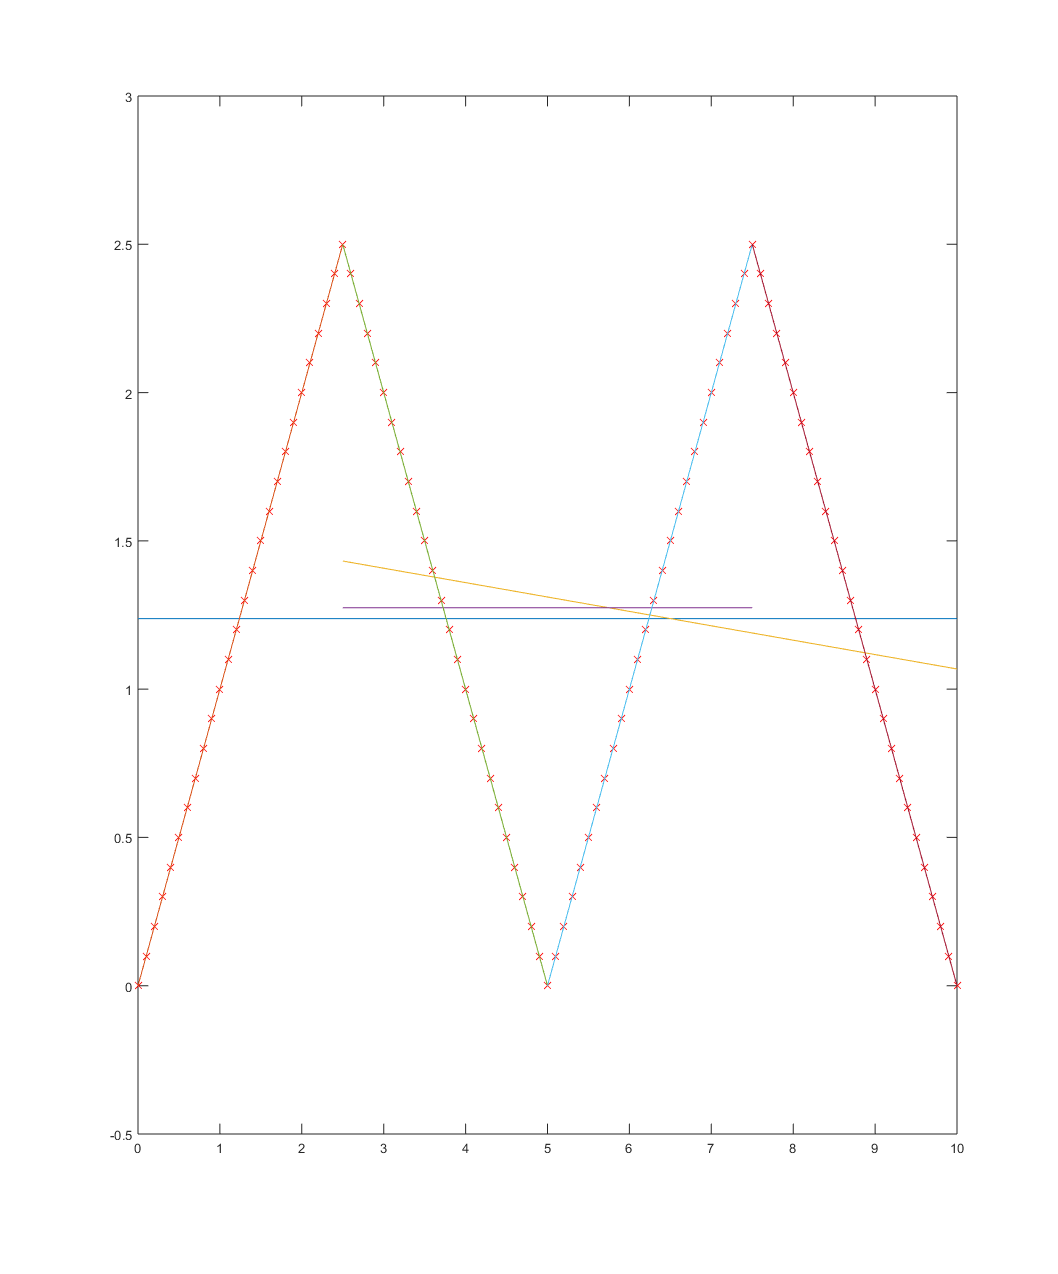
\includegraphics[scale=0.25]{q106_5}\\
					\caption[\textit{RPYAxes}]{Test 06 Stepped Through}
				\end{centering}
			\end{figure}
			\newline			
			
			\begin{figure}[position = here]
				\begin{centering}
					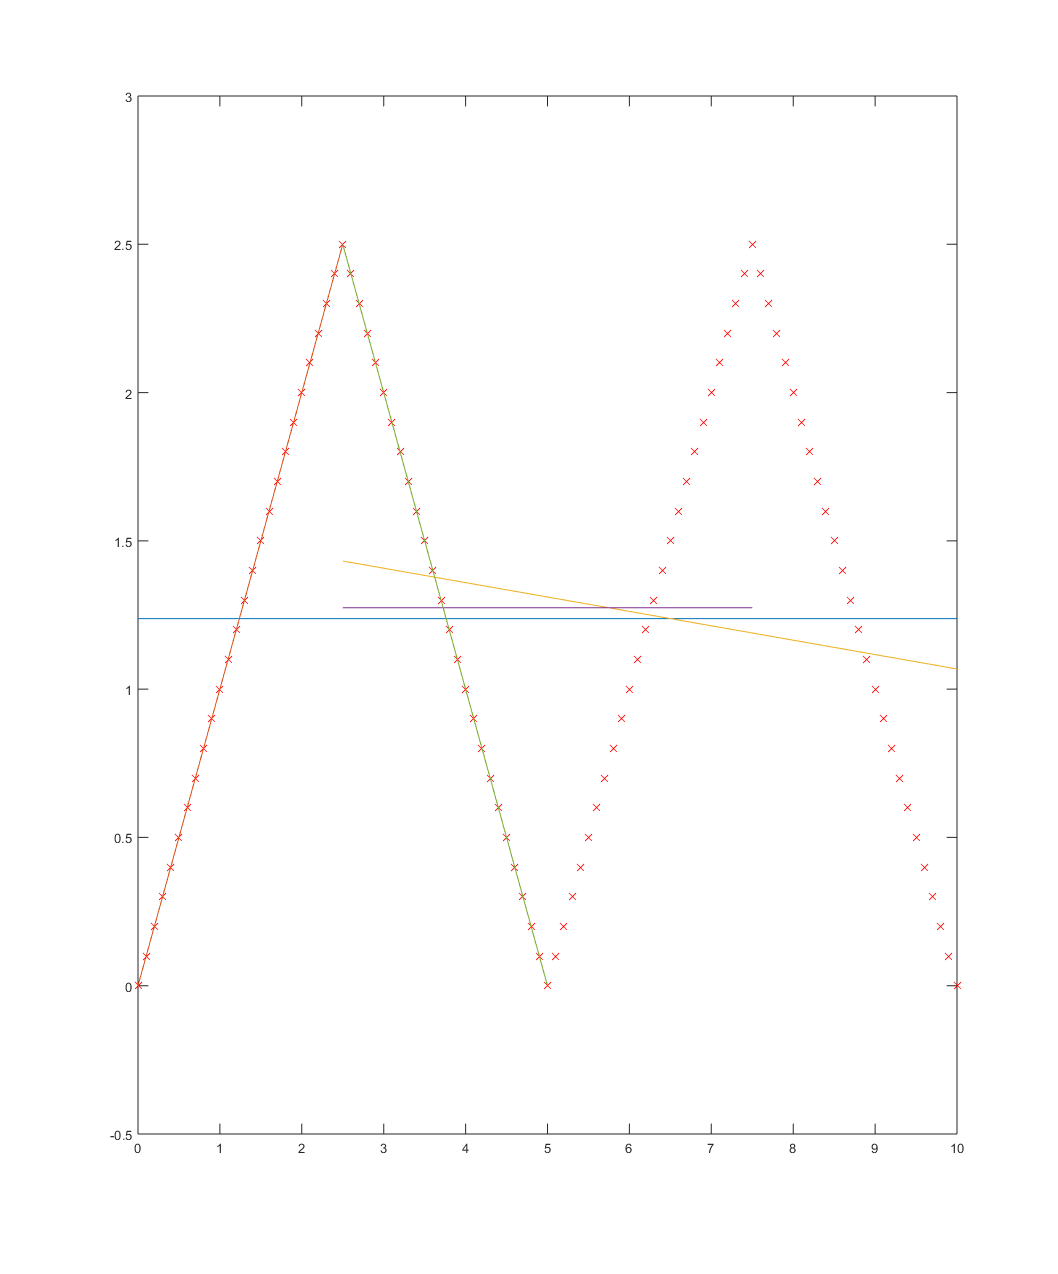
\includegraphics[scale=0.25]{q106_6}\\
					\caption[\textit{RPYAxes}]Test 06 Stepped Through}
				\end{centering}
			\end{figure}
			\newline								
			
			\begin{figure}[position = here]
				\begin{centering}
					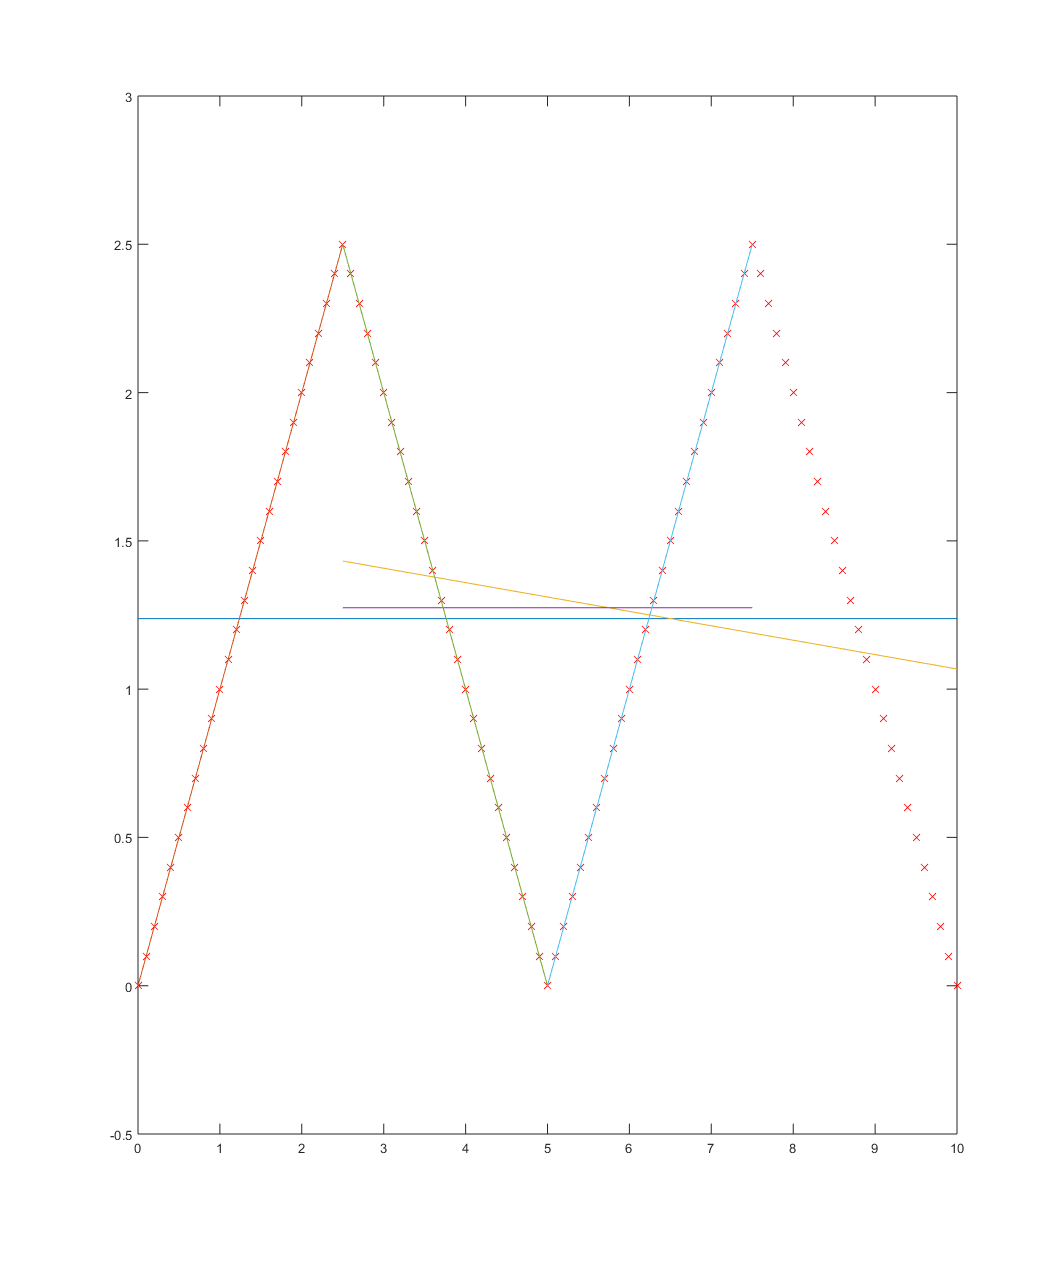
\includegraphics[scale=0.25]{q106_7}\\
					\caption[\textit{RPYAxes}]{Test 06 Stepped Through}
				\end{centering}
			\end{figure}
			\newline										

	\pagebreak
	\subsection{Laser Show ACFR Line Fitting}	%d
			\lstinputlisting{./code/Q1/laserShowACFR.m}
			\linebreak
			\begin{figure}[position = here]
				\begin{centering}
					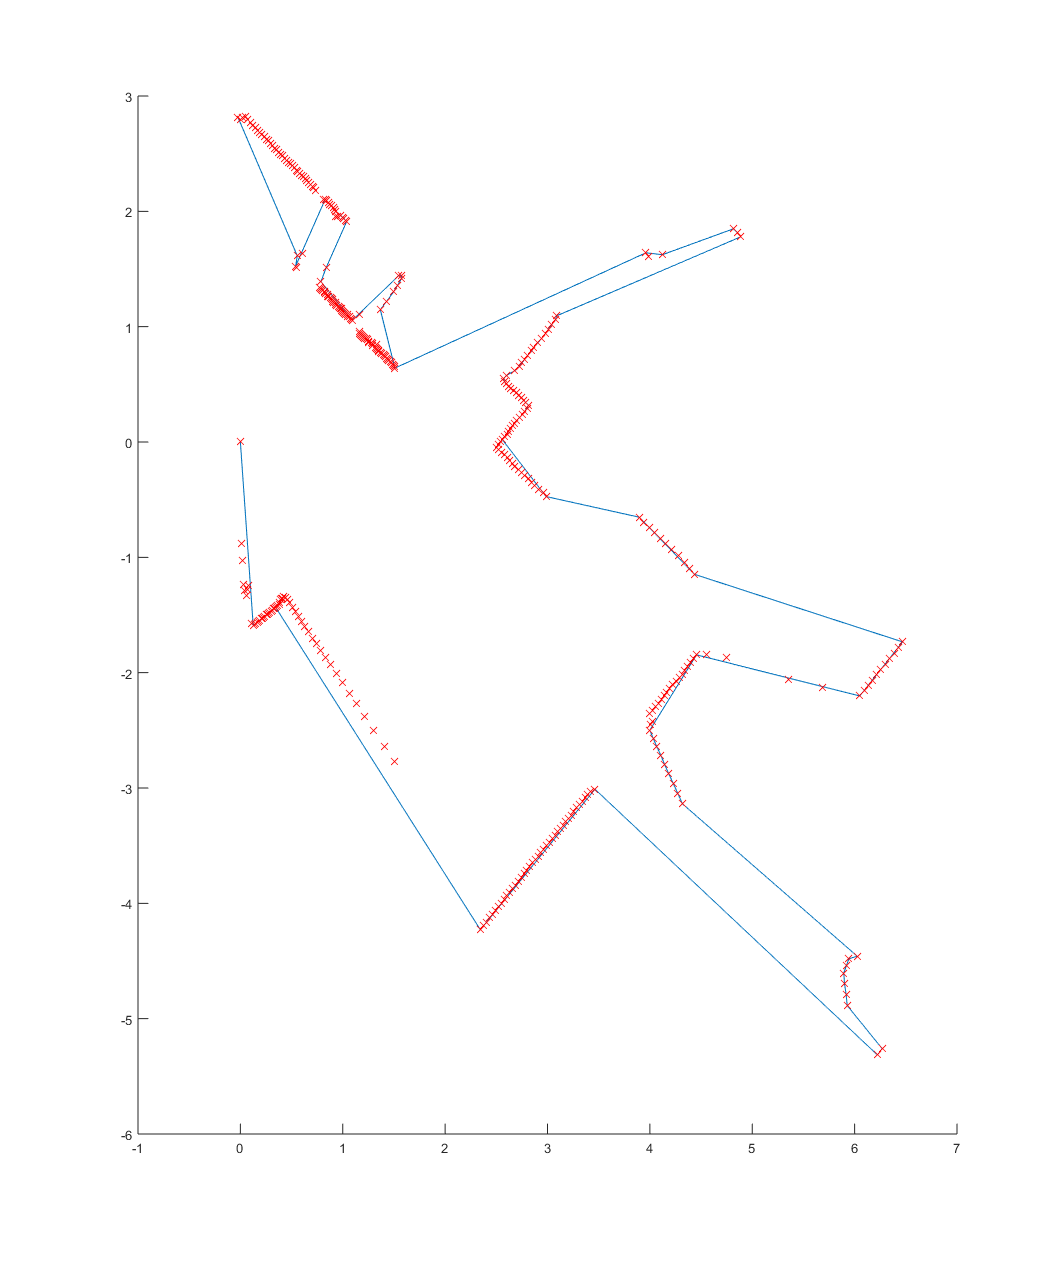
\includegraphics[scale=0.2]{q1d_solution}\\
					\caption[\textit{RPYAxes}]{LaserShowACFR approximate}
				\end{centering}
			\end{figure}
			\newline	
			
	\pagebreak
	\subsection{Corner Detection}	%e
		\lstinputlisting{./code/Q1/findcorners.m}
		\linebreak
		
		\begin{figure}[position = here]
			\begin{centering}
				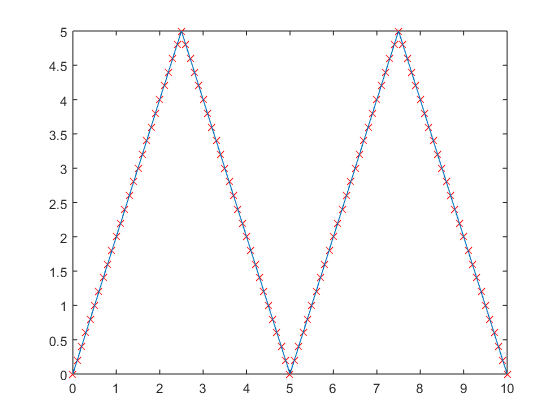
\includegraphics[scale=0.5]{q1_test10}\\
				\caption[\textit{RPYAxes}]{Non-Perpendicular Zig Zag Corner Test}
			\end{centering}
		\end{figure}
		\newline
		
		\begin{figure}[position = here]
			\begin{centering}
				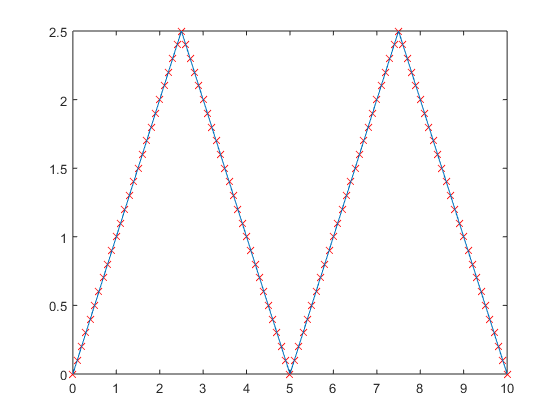
\includegraphics[scale=0.5]{q1_test11}\\
				\caption[\textit{RPYAxes}]{Perpendicular Zig Zag Corner Test}
			\end{centering}
		\end{figure}
		\newline		
		\pagebreak
		\lstinputlisting{./code/Q1/test/Q1test_results/test_results.txt}
		\linebreak
		
		As you can see the corners listed match perfectly with those graphed on Fig 21 (Test 11).
		
		\lstinputlisting{./code/Q1/q1e.txt}
		\linebreak
		The above corner values relate to the plot of the line estimates of the Laser Show ACFR scan in figure 19.
		
		\subsection*{Test Code Listing}
			See Appendix A [9.1]